\chapter{Vícero náhodných proměnných}

\section{Sdružená pravděpodobnost}

\subsection{Sdružená kumulativní distribuční funkce}

\begin{definition}[Sdružená kumulativní distribuční funkce]
Nechť jsou $X_1, X_2, ..., X_k$ náhodné veličiny definované nad pravděpodobnostním prostorem $(\Omega, \mathscr{A}, P[\cdot])$. Sdružená kumulativní distribuční funkce $F_{X_1, ..., X_k}(\cdot, ..., \cdot)$ je definována jako $P[X_1 \le x_1, ..., X_k \le x_k]$ pro všechna $x_1, x_2, ..., x_k$.
\end{definition}

Sdružená kumulativní distribuční funkce je tak funkcí s definičním oborem $R^k$ a intervalem $[0, 1]$ jako oborem hodnot.

\subsubsection{Dvourozměrná sdružená kumulativní distribuční funkce}

\begin{theorem}
Dvourozměrná sdružená kumulativní distribuční funkce splňuje následující podmínky.
~
\begin{enumerate}
\item
\begin{gather*}
F(-\infty, y) = \lim_{x \rightarrow -\infty}F(x, y) = 0 ~~~\textit{pro všechna}~y\\
F(x, -\infty) = \lim_{y \rightarrow -\infty}F(x, y) = 0 ~~~\textit{pro všechna}~x\\
F(\infty, \infty) = \lim_{x \rightarrow \infty, y \rightarrow \infty}F(x, y) = 1
\end{gather*}
\item Jestliže $x_1 < x_2$ a $y_1 < y_2$, pak $P[x_1 < X \le x_2, y_1 < Y \le y_2] = F(x_2, y_2) - F(x_2, y_1) - F(x_1, y_2) + F(x_1, y_1) \ge 0$.
\item Funkce $F(x,y)$ je v obou parametrech zprava spojitá. To znamená, že $\lim_{0 < h \rightarrow 0}F(x + h, y) = \lim_{0 < h \rightarrow 0}F(x, y + h) = F(x, y)$.
\end{enumerate}
\end{theorem}

\begin{definition}[Dvourozměrná kumulativní distribuční funkce]
Libovolná funkce, která splňuje výše uvedené tři podmínky, je dvourozměrnou kumulativní distribuční funkcí.
\end{definition}

\begin{definition}[Marginální kumulativní distribuční funkce]
Jestliže je $F_{X,Y}(\cdot, \cdot)$ sdruženou kumulativní distribuční funkcí náhodných veličin $X$ a $Y$, pak kumulativní distribuční funkce $F_X(\cdot)$ a $F_Y(\cdot)$ jsou její marginální kumulativní distribuční funkce.
\end{definition}

\begin{corollary}
Platí $F_X(x) = F_{X,Y}(x, \infty)$ a $F_Y(y) = F_{X,Y}(\infty, y)$. Známe-li sdruženou kumulativní distribuční funci, jsme schopni určit také odpovídající marginální kumulativní distribuční funkce. 
\end{corollary}

Obrácené tvrzení však neplatí - znalost marginálních kumulativních distribučních funkcí neimplikuje znalost sdružené kumulativní distribuční funkce.

\begin{theorem}
V případě dvourozměrné sdružené kumulativní distribuční funkce pro všechna $x$ a $y$ platí
\begin{equation*}
F_X(x) + F_Y(y) - 1 \le F_{X,Y}(x,y) \le \sqrt{F_X(x)F_Y(y)}
\end{equation*}
\end{theorem}

\begin{proof}
Nejprve dokážeme
\begin{equation*}
F_X(x) + F_Y(y) - 1 \le F_{X,Y}(x,y)
\end{equation*}
Levou stranu této nerovnosti lze upravit do podoby
\begin{gather*}
1 - P[x < X < \infty, y < Y < \infty] + F_{X,Y} - 1\\
= F_{X,Y} - P[x < X < \infty, y < Y < \infty]
\end{gather*}
Protože $P[x < X < \infty, y < Y < \infty] \ge 0$, platí $F_X(x) + F_Y(y) - 1 \le F_{X,Y}(x,y)$. Následně dokážeme
\begin{equation*}
F_{X,Y}(x,y) \le \sqrt{F_X(x)F_Y(y)}
\end{equation*}
Tuto nerovnost lze upravit do podoby
\begin{gather*}
\ln \big(F_{X,Y}(x,y) \big) + \ln \big( F_{X,Y}(x,y) \big) \le \ln \big(F_x(x) \big) + \ln \big( F_Y(y) \big)
\end{gather*}
Protože $F_{X,Y}(x,y) \le F_X(x)$ a $F_{X,Y}(x,y) \le F_Y(y)$, výše uvedená nerovnost platí, čímž uzavíráme důkaz.
\end{proof}

\subsection{Sdružená pravděpodobnostní funkce nespojité náhodné veličiny}

Jestliže jsou $X_1, X_2, ..., X_k$ náhodné veličiny definované nad shodným pravděpodobnostním prostorem, pak je $(X_1, X_2, ..., X_k)$ $n$-rozměrnou náhodnou veličinou.

\begin{definition}[Sdružená nespojitá náhodná veličina]
Náhodná veličina $(X_1, X_2, ..., X_k)$ je $k$-rozměrnou nespojitou náhodnou veličinou, jestliže může nabývat hodnot pouze nad spočetným množstvím bodů $(x_1, x_2, ..., x_k)$ z $R^k$.
\end{definition}

\begin{definition}[Sdružená nespojitá pravděpodobnostní funkce]
Jestliže $(X_1, X_2, ..., X_k)$ je $k$-rozměrná nespojitá náhodná veličina, pak její sdružená nespojitá pravděpodobnostní funkce $f_{X_1, X_2, ..., X_k}(\cdot, ..., \cdot)$ je definována pro hodnoty $(x_1, x_2, ..., x_k)$, kterých může náhodná veličina $(X_1, X_2, ..., X_k)$ nabývat, jako
\begin{equation*}
f_{X_1, X_2, ..., X_k} = P[X_1 = x_1, X_2 = x_2, ..., X_k = x_k]
\end{equation*}
V ostatních případech je tato funkce rovna nule.
\end{definition}
Stejně jako v případě jednorozměrné náhodné veličiny také v případě $k$-rozměrné náhodné veličiny platí $\sum f_{X_1, X_2, ..., X_k}(x_1, x_2, ..., x_k) = 1$, kde sčítáme přes všechny přípustné hodnoty náhodné veličiny $(X_1, X_2, ..., X_k)$.

\begin{theorem}
Jestliže $X$ a $Y$ jsou sdruženě nespojité náhodné veličiny, pak znalost $F_{X,Y}(\cdot, \cdot)$ je ekvivalentní znalosti $f_{X,Y}(\cdot, \cdot)$. Toto tvrzení lze zobecnit také na $k$-rozměrnou náhodnou veličinu.
\end{theorem}

\begin{proof}
Nechť $(x_1, y_1), (x_2, y_2), ...$ představují všechny možné hodnoty náhodné veličiny $(X, Y)$. Jestliže známe $f_{X,Y}$, pak
\begin{equation*}
F_{X,Y}(x,y) = \sum f_{X,Y}(x_i, y_i)
\end{equation*}
kde sčítáme přes všechna $i$, pro která $x_i \le x$ a $y_i \le y$. Naopak je-li dáno $F_{X,Y}(\cdot, \cdot)$ pro všechna $(x_i, y_i)$, pak
\begin{equation*}
f_{X,Y}(x_i, y_i) = F_{X,Y}(x_i, y_i) - \lim_{0 < h \rightarrow 0} F_{X,Y}(x_i - h, y_i) - \lim_{0 < h \rightarrow 0}F_{X,Y}(x_i, y_i - h)
\end{equation*}
\end{proof}

\begin{definition}[Marginální nespojitá pravděpodobnostní funkce]
Jestliže jsou $X$ a $Y$ sdružené nespojité náhodné veličiny, pak $f_X(\cdot)$ a $f_Y(\cdot)$ představují marginální pravděpodobnostní funkce. Tuto definici lze zobecnit. Nechť $X_{i_1}, ..., X_{i_m}$ představují libovolnou podmnožinu sdružených nespojitých náhodných veličin $X_1, ..., X_k$. Pak $f_{X_{i_1}, ..., X_{i_m}}(x_{i_1}, ..., x_{i_m})$ představuje marginální pravděpodobnostní funkci. 
\end{definition}

Jestliže jsou $X_1, ..., X_k$ sdružené nespojité náhodné veličiny, pak lze libovolnou marginální pravděpodobnostní funkci odvodit ze sdružené pravděpodobnostní funkce. Obrácené tvrzení však neplatí.

\begin{example}
Uvažujme hod dvěma čtyřstěny. Náhodná veličina $X$ značí hodnotu hodu prvního z nich. Náhodná veličina $Y$ pak značí největší z obou hodů. Předpokládejme, že tyto čtyřstěny nejsou dokonale vyvážené, a proto se skutečně realizované pravděpodobnosti liší od očekávaných. Jednu z možných situací zachycuje následující tabulka.
\begin{center}
  \begin{tabular}{|c|c|c|c|c|}
    \hline
    $4$ & $1/16 + \epsilon$ &  $1/16 - \epsilon$ & $1/16$ & $4/16$\\
    \hline
    $3$ & $1/16 - \epsilon$ &  $1/16 + \epsilon$ & $3/16$ & $0$\\
    \hline
    $2$ & $1/16$ &  $2/16$ & $0$ & $0$\\
    \hline
    $1$ & $1/16$ &  $0$ & $0$ & $0$\\
    \hline
    $y/x$ & $1$ & $2$ & $3$ & $4$\\
    \hline
  \end{tabular}
\end{center}
Pro libovolné $0 \le \epsilon \le \frac{1}{16}$ definuje tato tabulka sdruženou pravděpodobnostní funkci. Nicméně marginální pravděpodobnosti jsou nezávislé na $\epsilon$. Tento příklad tedy ilustruje, že znalost marginálních pravděpodobnostních funkcí neimplikuje znalost sdružené pravděpodobnostní funkce.
\end{example}

Uvažujme experiment, který má $k+1$ možných výsledků. Označme tyto výsledky jako $s_1, s_2, ...,s_{k+1}$. Definujme $p_i = P[s_i]$ pro $i = 1, ..., k+1$. Je zřejmé, že musí platit $\sum_{i = 1}^{k + 1}p_i = 1$. Předpokládejme, že tento pokus opakujeme $n$-krát a že jednotlivé pokusy jsou vzájemně nezávislé. Nechť náhodná velčina $X_i$ představuje počet realizací $s_i$. Nespojitá pravděpodobnostní funkce náhodných veličin $X_1, ..., X_k$ je definována jako
\begin{equation*}
f_{X_1, ..., X_k}(x_1, ..., x_k) = \frac{n!}{\prod_{i = 1}^{k + 1}x_i!}\prod_{i = 1}^{k + 1}p_i^{x_i}
\end{equation*}
kde $x_i = 0, ..., n$ a $\sum_{i = 1}^{k + 1} x_i = n$. Všimněme si, že platí $X_{k+1} = n - \sum_{i = 1}^k X_i$.

Výše uvedenou rovnici lze vysvětlit následovně. Levou stranu této rovnice je možné vyjádřit ve tvaru $P[X_1 = x_1, ..., X_{k + 1} = x_{k + 1}]$. Zajímá nás tak pravděpodobnost, že mezi $n$ vzájemně nezávislými pokusy bude právě $x_1$ realiací $s_1$,  $x_2$ realizací $s_2$ až $x_{k + 1}$ realiací $s_{k + 1}$, kde $\sum_1^{k+1}x_i = n$. Za předpokladu nezávislosti jednotlivých pokusů lze pravděpodobnost jednoho takovéhoto uspořádání vyjádřit jako $p_1^{x_1}p_2^{x_2} \cdots p_{k+1}^{x_k + 1}$. Takovýchto uspořádání pak existuje $\frac{n!}{x_1!x_2! \cdots x_{k+1}!}$.

\begin{definition}[Multinomiální rozdělení]
Výše uvedená sdružená nespojitá pravděpodobnostní funkce se nazývá multinomiální distribucí.
\end{definition}

Multinomiální rozdělení má $(k + 1)$ parametrů a to $n, p_1, p_2, ..., p_k$. Parametr $p_{k+1}$ je definován jako $1 - p_1 - p_2 - ... - p_k$. Marginální rozdělení náhodné veličiny $X_i$ má charakter binomického rozdělení s parametry $n$ a $p_i$, protože na výsledek každého experimentu je možné pohlížet jako realizaci popř. nerealizaci výsledku $s_i$. Na každý z $n$ pokusů je tak možné pohlížet jako na Bernoulliho pokus a na sérii $n$ pokusů je pak možné modelovat pomocí binomického rozdělení.

\subsection{Sdružená pravděpodobnostní funkce spojité náhodné veličiny}

\begin{definition}[Sdružená spojitá náhodná veličina a její pravděpodobnostní funkce]
$k$-rozměrná náhodná veličina $(X_1, X_2, ..., X_k)$ je $k$-rozměrnou náhodnou veličinou právě tehdy a jen tehdy, jestliže existuje funkce $f_{X_1, ..., X_k}(\cdot, ..., \cdot) \ge 0$ taková, že
\begin{equation*}
F_{X_1, ..., X_k}(x_1, ..., x_k) = \int_{-\infty}^{x_k} \cdots \int_{-\infty}^{x_1} f_{X_1, ..., X_k}(u_1, ..., u_k)du_1 \cdots du_k
\end{equation*}
pro všechna $(x_1, ..., x_k)$. Funkce $f_{X_1, ..., X_k}(\cdot, ..., \cdot)$ je tzv. sdruženou pravděpodobnostní funkcí. Tato funkce splňuje následující dvě podmínky.
\begin{enumerate}
\item $f_{X_1, ..., X_k}(x_1, ..., x_k) \ge 0$
\item $\int_{-\infty}^{\infty} \cdots \int_{-\infty}^{\infty} f_{X_1, ..., X_k}(x_1, ..., x_k)dx_1 \cdots dx_k = 1$
\end{enumerate}
\end{definition}

\begin{example}
Uvažujme funkci
\begin{equation*}
f(x,y) = K(x + y)I_{(0, 12)}(x)I_{(0,1)}(y)
\end{equation*}
Lze vhodně zvolit konstantu $K$ tak, aby tato funkce byla dvourozměrnou pravděpodobnostní funkcí?

\begin{gather*}
\int_{-\infty}^{\infty} \int_{-\infty}^{\infty} K(x + y)dx dy = K \int_0^1 \int_0^1 (x + y)dx dy\\
=K \int_0^1 \big(\frac{1}{2} + y \big)dy = K \big(\frac{1}{2} + \frac{1}{2} \big) = 1
\end{gather*}
pro $K = 1$. Proto je funkce $f(x,y) = (x + y) I_{(0,1)}(x)I_{(0,1)}(y)$ sdruženou pravděpodobnostní funkcí.
\end{example}

\begin{theorem}
Jestliže jsou $X$ a $Y$ sdružené spojité náhodné veličiny, pak znalost sdružené kumulativní distribuční funkce $F_{X,Y}(\cdot, \cdot)$ je ekvivalentní znalosti sdružené pravděpodobnostní funkce $f_{X,Y}(\cdot, \cdot)$. Tuto větu lze rozšířit také na $k-$rozměrné spojité náhodné veličiny.
\end{theorem}
\begin{proof}
Pro danou sdruženou pravděpodobnostní funkci $f_{X,Y}(\cdot, \cdot)$ lze pro libovolné $(x,y)$ odvodit sdruženou kumulativní distribuční funkci $F_{X,Y}(x,y)$ jako
\begin{equation*}
F_{X,Y}(x,y) = \int_{-\infty}^y \int_{-\infty}^x f_{X,Y}(u,v)du dv
\end{equation*}
Naopak, pro danou sdruženou kumulativní distribuční funkci $F_{X,Y}(x,y)$ lze odpovídající sdruženou pravděpodobnostní funkci $f_{X,Y}(\cdot, \cdot)$ odvodit jako
\begin{equation*}
f_{X,Y}(x,y) = \frac{\partial^2 F_{X,Y}(x,y)}{\partial x \partial y}
\end{equation*}
kde $x$ a $y$ představují body, pro které je $F_{X,Y}(x,y)$ derivovatelná.
\end{proof}

\begin{definition}[Marginální pravděpodobnostní funkce]
Jestliže jsou $X$ a $Y$ sdružené spojité náhodné veličiny, pak $f_X(\cdot)$ a $f_Y(\cdot)$ jsou nazývány marginálními pravděpodobnostními funkcemi.

Tuto definici lze zobecnit. Nechť $X_{i_1}, ..., X_{i_m}$ představuje libovolnou podmnožinu sdružených náhodných veličin $X_1, ..., X_k$. Pak je funkce $f_{X_{i_1}, ..., X_{i_m}}(x_{i_1}, ..., x_{i_m})$ je nazývána marginální pravděpodobnostní funkcí náhodné veličiny $(X_{i_1}, ..., X_{i_m})$.
\end{definition}

Jestliže jsou $X$ a $Y$ sdružené spojité náhodné veličiny, pak platí
\begin{equation*}
f_X(x) = \int_{-\infty}^{\infty} f_{X,Y}(x,y)dy
\end{equation*}
a
\begin{equation*}
f_Y(y) = \int_{-\infty}^{\infty} f_{X,Y}(x,y)dx
\end{equation*}
protože
\begin{equation*}
f_X(x) = \frac{d F_X(x)}{dx} = \frac{d}{dx}\Big[\int_{-\infty}^x \Big(\int_{-\infty}^{\infty}f_{X,Y}(u,y)dy \Big) du \Big] = \int_{-\infty}^{\infty} f_{X,Y}(x,y)dy
\end{equation*}
a
\begin{equation*}
f_Y(y) = \frac{d F_Y(y)}{dy} = \frac{d}{dy}\Big[\int_{-\infty}^x \Big(\int_{-\infty}^{\infty}f_{X,Y}(x,u)dx \Big) du \Big] = \int_{-\infty}^{\infty} f_{X,Y}(x,y)dx
\end{equation*}

\begin{example}
Uvažujme sdruženou pravděpodobnostní funkci
\begin{equation*}
f_{X,Y}(x,y) = (x + y)I_{(0,1)}(x) I_{(0, 1)}(y)
\end{equation*}
Sdruženou kumulativní distribuční funkci lze vypočíst následujícím způsobem.
\begin{gather*}
F_{X,Y}(x,y) = I_{(0,1)}(x) I_{(0, 1)}(y) \int_0^y \int_0^x (u + v)du dv + I_{(0,1)}(x)I_{[1, \infty)}(y) \int_0^1 \int_0^x (u + v)du dv\\
+ I_{[1, \infty)}(x)I_{(0,1)}(y) \int_0^y \int_0^1 (u + v) du dv + I_{[1, \infty)}(x)I_{[1, \infty)}(y)\\
= \frac{1}{2}[(x^2y + xy^2)I_{(0,1)}(x)I_{(0,1)}(y) + (x^2 + x)I_{(0, 1)}(x)I_{[1, \infty)}(y)\\
+ (y + y^2)I_{[1, \infty)}(x)I_{(0, 1)}(y)] + I_{[1, \infty)}(x)I_{[1, \infty)}(y)
\end{gather*}
Marginální pravděpodobnostní funkci pak lze vyjádřit jako
\begin{gather*}
f_X(x) = \int_{-\infty}^{\infty} f_{X,Y}(x,y)dy = I_{(0, 1)}(x) \int_0^1(x+y)dy = \big(x + \frac{1}{2} \big)I_{(0, 1)}(x)
\end{gather*}
popř. jako
\begin{gather*}
f_X(x) = \frac{\partial F_{X,Y}(x, \infty)}{\partial x} = \frac{\partial F_X(x)}{\partial x} = I_{(0,1)}(x) \frac{\partial}{\partial x} \Big(\frac{x^2 + x}{2} \Big) = \big(x + \frac{1}{2} \big)I_{(0, 1)}(x)
\end{gather*}
\end{example}

\section{Podmíněné rozdělení a nezávislost}

\subsection{Podmíněná kumulativní distribuční funkce nespojité náhodné veličiny}

\begin{definition}[Podmíněná nespojitá pravděpodobnostní funkce]
Nechť jsou $X$ a $Y$ sdružené nespojité náhodné veličiny se sdruženou nespojitou pravděpodobnostní funkcí $f_{X,Y}(\cdot, \cdot)$. Podmíněná nespojitá pravděpodobnostní funkce $f_{Y|X}(\cdot | x)$ náhodné veličiny $Y$ pro $X = x$ je definována jako
\begin{equation*}
f_{Y|X}(y|x) = \frac{f_{X,Y}(x,y)}{f_X(x)}
\end{equation*}
je-li $f_X(x) > 0$, kde $f_X(x)$ je marginální pravděpodobnostní funkce náhodné veličiny $X$ v bodě $x$. Pro $f_X(x) = 0$ není funkce $f_{Y|X}(\cdot | x)$ definována. Podobně
\begin{equation*}
f_{X|Y}(x|y) = \frac{f_{X,Y}(x,y)}{f_Y(y)}
\end{equation*}
za podmínky $f_Y(y) > 0$.
\end{definition}

Protože náhodné veličiny $X$ a $Y$ jsou nespojité, mohou nabývat hodnot některého z bodů koncentrace $x_1, x_2,...$ v případě $X$ a $y_1, y_2, ...$ v případě $Y$. Jestliže $f_X(x) > 0$, pak $x = x_i$ pro některé $i$ a $f_X(x_i) = P[X = x_i]$. Analogicky $f_{X,Y}(x_i, y_i) = P[X = x_i, Y = y_j]$. Proto
\begin{equation*}
f_{Y|X}(y_j|x_i) = \frac{f_{X,Y}(x_i, y_j)}{f_X(x_i)} = \frac{P[X = x_i, Y = y_j]}{P[X = x_i]} = P[Y = y_j | X = x_i]
\end{equation*}
Jedná se tedy o podmíněnou pravděpodobnost, tak jak jsme ji definovali v první kapitole.

Vzhledem k tomu, že $f_{Y|X}(y_j|x_i)$ je nespojitá distribuční funkce, musí být kladná a její součet přes všechny přípustné hodnoty $Y$ musí být roven jedné. První podmínka je splněna, protože $f_{X,Y}(x,y)$ je nezáporné a $f_X(x)$ je kladné, a proto je jejich podíl kladný. Druhá podmínka je taktéž splněna, protože
\begin{equation*}
\sum_j f_{Y|X}(y_j|x) = \sum_j \frac{f_{X,Y}(x, y_j)}{f_X(x)} = \frac{1}{f_X(x)} \sum_j f_{X,Y}(x,y_j) = \frac{f_X(x)}{f_X(x)} = 1
\end{equation*} 

\begin{definition}[Podmíněná nespojitá kumulativní distribuční funkce]
Jestliže jsou $X$ a $Y$ sdružené nespojité náhodné veličiny, pak podmíněná nespojitá kumulativní distribuční fukce $F_{Y|X}(\cdot | x)$ je definována jako $F_{Y|X}(y|x) = P[Y \le y | X = x]$ pro $f_X(x) > 0$. Vazba mezi podmíněnou nespojitou kumulativní distribuční funkcí a pravděpodobnostní funkcí je dána vztahem
\begin{equation*}
F_{Y|X}(y|x) = \sum_{j:y_j \le y} f_{Y|X}(y_j | x)
\end{equation*}
\end{definition}

\begin{definition}[Podmíněná nespojitá pravděpodobnostní funkce]
Nechť $(X_1, ..., X_k)$ je $k$-rozměrná nespojitá náhodná veličina a nechť $X_{i_1}, ..., X_{i_r}$ a $X_{j_1}, ..., X_{j_s}$ jsou dvě neslučitelné podmnožiny náhodných veličin $X_1, ..., X_k$. Podmíněná pravděpodobnostní funkce $r$-rozměrné náhodné veličiny $X_{i_1}, ..., X_{i_r}$ pro dané hodnoty $(x_{j_1}, ..., x_{j_s})$ náhodné veličiny $X_{j_1}, ..., X_{j_s}$ je definována jako
\begin{gather*}
f_{X_{i_1}, ..., X_{i_r}|x_{j_1},...,x_{j_s}}(x_{i_1}, ..., x_{i_r}|x_{j_1}, ..., x_{j_s})\\
= \frac{f_{X_{i_1}, ..., X_{i_r}, X_{j_i}, ..., X_{j_s}}(x_{i_1}, ..., x_{i_r}, x_{j_1}, ..., x_{j_s})}{f_{X_{j_1}, ..., X_{j_s}}(x_{j_1}, ..., x_{j_s})}
\end{gather*}
\end{definition}

\begin{example}
Vyberme 12 karet bez vracení ze standardního hracího balíčku. Nechť $X_1$ představuje počet tažených es, $X_2$ představuje počet tažených dvojek, $X_3$ představuje počet tažených trojek a $X_4$ počet tažených čtyřek. Sdružená pravděpodobnostní funkce těchto čtyř náhodných veličin je
\begin{equation*}
f_{X_1, X_2, X_3, X_4}(x_1, x_2, x_3, x_4) = \frac{\binom{4}{x_1}\binom{4}{x_2}\binom{4}{x_3}\binom{4}{x_4}\binom{36}{12 - x_1 - x_2 - x_3 - x_4}}{\binom{52}{12}}
\end{equation*}
kde $x_i = 0, 1, 2, 3, 4$ při omezení $\sum x_i \le 12$. Existuje velké množství souvisejících podmíněných pravděpodobnostních funkcí. Jednou z nich je např.
\begin{gather*}
f_{X_2, X_4 | X_1, X_3}(x_2, x_4 | x_1, x_3)\\
= \frac{\binom{4}{x_1}\binom{4}{x_2}\binom{4}{x_3}\binom{4}{x_4}\binom{36}{12 - x_1 - x_2 - x_3 - x_4} \Big/ \binom{52}{12}}{\binom{4}{x_1}\binom{4}{x_3}\binom{44}{12 - x_1 - x_3} \Big/ \binom{52}{12}}\\
= \frac{\binom{4}{x_2}\binom{4}{x_4}\binom{36}{12 - x_1 - x_2 - x_3 - x_4} \Big/ \binom{52}{12}}{\binom{44}{12 - x_1 - x_3} \Big/ \binom{52}{12}}
\end{gather*}
\end{example}

\subsection{Podmíněná pravděpodobnostní funkce spojitých náhodných veličin}

\begin{definition}[Podmíněná pravděpodobnostní funkce]
Nechť jsou $X$ a $Y$ sdružené spojité náhodné veličiny se sdruženou pravděpodobnostní funkcí $f_{X,Y}(x,y)$. Podmíněná pravděpodobnostní funkce náhodné veličiny $Y$ pro $X = x$ je definována jako
\begin{equation*}
f_{Y|X}(y|x) = \frac{f_{X,Y}(x,y)}{f_X(x)}
\end{equation*}
kde $f_X(x) > 0$. Pro $f_X(x) > 0$ není tato funkce definována. Podobně $f_{X|Y}(x|y)$ je definována jako
\begin{equation*}
f_{X|Y}(x|y) = \frac{f_{X,Y}(x,y)}{f_Y(y)}
\end{equation*}
pro $f_Y(y) > 0$ a nedefinováno pro $f_Y(y) = 0$.
\end{definition}

Funkce $f_{Y|X}(\cdot | x)$ se nazývá podmíněná pravděpodobnostní funkce a proto by měla být nezáporná a její integrál přes všechny přípustné hodnoty by měl být roven jedné. První podmínka je splněna, protože $f_{X,Y}(x,y)$ je nezáporné a $f_Y(y)$ je kladné. Druhá podmínka je taktéž splněna, protože
\begin{gather*}
\int_{-\infty}^{\infty} f_{Y|X}(y|x)dy = \int_{-\infty}^{\infty} \frac{f_{X,Y}(x,y)}{f_X(x)}dy\\
= \frac{1}{f_X(x)} \int_{-\infty}^{\infty} f_{X,Y}(x,y)dy = \frac{f_X(x)}{f_X(x)} = 1
\end{gather*}

Uvažujme $f_{Y|X}(\cdot | x_0)$. Funkci $f_{X,Y}(x,y)$ lze znároznit jako plochu nad rovinou $xy$. Rovina kolmá na rovinu $xy$, která ji protíná v přímce $x = x_0$, protíná plochu $f_{X,Y}(x,y)$ v křivce $f_{X,Y}(x_0,y)$. Plocha pod toutu křivkou je
\begin{equation*}
\int_{-\infty}^{\infty}f_{X,Y}(x_0, y)dy = f_X(x_0)
\end{equation*}
Proto, vydělíme-li $f_{X,Y}(x_0,y)$ touto plochou $f_X(x_0)$, získáme pravděpodobnostní funkce $f_{Y|X}(y|x_0)$.

\begin{definition}[Podmíněná spojitá kumulativní distribuční funkce]
Jestliže jsou $X$ a $Y$ sdružené spojité náhodné veličiny, pak je podmíněná kumulativní distribuční funkce náhodné veličiny $Y$ pro $X = x$ definována jako
\begin{equation*}
F_{Y|X}(y|x) = \int_{-\infty}^y f_{Y|X}(z|x)dz
\end{equation*}
pro všechna taková $x$, kde $f_X(x) > 0$.
\end{definition}

\begin{example}
Uvažujme sdruženou pravděpodobnostní funkci
\begin{equation*}
f_{X,Y}(x,y) = (x + y)I_{(0,1)}(x)I_{(0,1)}(y)
\end{equation*}
Podmíněnou pravděpodobnostní funkci pak lze vypočíst jako
\begin{equation*}
f_{Y|X}(y|x) = \frac{(x + y)I_{(0, 1)}(x)I_{0, 1}(y)}{\Big(x + \frac{1}{2} \Big)I_{(0, 1)}(x)} = \frac{x + y}{x + \frac{1}{2}} I_{(0, 1)}(y)
\end{equation*}
pro $0 < x < 1$. Kumulativní distribuční funkci pak lze odvodit jako
\begin{equation*}
F_{Y|X}(y|x) = \int_{-\infty}^y f_{Y|X}(z|x)dz = \int_0^y \frac{x + z}{x + \frac{1}{2}}dz\\
= \frac{1}{x + \frac{1}{2}} \int_0^y (x + z) dz = \frac{1}{x + \frac{1}{2}}(xy + \frac{y^2}{2})
\end{equation*}
pro $0 < y < 1$.
\end{example}

Definici podmíněné pravděpodobnostní funkce lze analogicky rozšířit také na $k$-rozměrnou spojitou náhodnou veličinu. Např.
\begin{equation*}
f_{X_1, X_2, X_4 | X_3, X_5}(x_1, x_2, x_4 | x_3, x_5) = \frac{f_{X_1, X_2, X_3, X_4, X_5}(x_1, x_2, x_3, x_4, x_5)}{f_{X_3, X_5}(x_3, x_5)}
\end{equation*}
pro $f_{X_3, X_5}(x_3, x_5) > 0$.

\subsection{Více o podmíněné pravděpodobnostní funkci}

Uvažujme pravděpodobnost náhodného jevu $A$ podmíněného $X = x$, kde $X$ může být jak spojitá tak nespojitá náhodná veličina. Předpokládejme, že jak náhodný jev $A$ tak náhodná veličina $X$ jsou definovány nad shodným pravděpodobnostním prostorem. Pokusme se definovat $P[A|X = x]$. Jestliže je $X$ nespojité a $x$ bodem koncentrace, pak
\begin{equation*}
P[A|X = x] = \frac{P[A, X = x]}{P[X = x]}
\end{equation*}
V opačném případě není $P[A, X = x]$ definováno. Jestliže je $X$ spojité, pak $P[X = x] = 0$. Jestliže je však $x$ takové, že jev $x - h < X < x + h$ má kladnou pravděpodobnost pro libovolné $h > 0$, pak
\begin{equation*}
P[A | X = x] = \lim_{0 < h \rightarrow 0} P[A | x-h < X < x + h]
\end{equation*}
za předpokladu existence limity.\

Pro podmíněnou pravděpodobnost platí následující tvrzení.
\begin{corollary}
~
\begin{enumerate}
\item $P[A] = \sum_{i = 1}^{\infty}P[A|X = x_i]f_x(x_i)$ jestliže $X$ je nespojité s body koncentrace $x_1, x_2, ...$
\item $P[A] = \int_{-\infty}^{\infty}P[A|X = x]f_x(x)dx$ jestliže je $X$ spojité
\item $P[A, X \in B] = \sum_{i: x_i \in B} P[A|X = x_i]f_x(x_i)$ jestliže $X$ je nespojité s body koncentrace $x_1, x_2, ...$
\item $P[A, X \in B] = \int_B P[A|X = x]f_X(x)dx$ jestliže je $X$ spojité
\item $P[A | X = x] = P[h(X,Y) \le z | X = x] = P[h(x,Y) \le z | X = x]$ kde $A = {h(X,Y) \le z}$ a $h(\cdot, \cdot)$ je funkcí dvou proměnných
\end{enumerate}
\end{corollary}

Z druhé rovnice vyplývá
\begin{equation*}
F_Y(y) = \int_{-\infty}^{\infty} F_{Y|X}(y|x)f_X(x)dx
\end{equation*}
kde $A = {Y \le y}$. Ze čtvrté rovnice pak vyplývá
\begin{equation*}
F_{X,Y}(x,y) = \int_{-\infty}^x F_{Y|X}(y|x')f_X(x')dx'
\end{equation*}
kde $A = {Y \le y}$ a $B = (-\infty, x]$.

V některých případech je snadné nalézt $P[A|X = x]$ a složité nalézt $P[A]$. Jestliže však známe $f_X(\cdot)$, lze $P[A]$ vypočíst na základě některé z výše uvedených rovnic. 

\begin{example}
Uvažujme tři náhodně zvolené body na obvodu jednotkového kruhu. Jaká je pravděpodobnost, že se všechny tři body budou nacházet na témže polokruhu?

První bod zvolíme jako orientační, a proto ho umístíme do bodu nula. Nechť $X$ představuje polohu druhého bodu a jev $A$ představuje situaci, kdy se všechny tři body nachází na témže polokruhu. Náhodná veličina $X$ sleduje uniformní rozdělení nad intervalem $(0, 2 \pi)$. Pro náhodný jev $A$ platí $P[A] = \int P[A|X = x]f_X(x)dx$. Je-li $0 < x < \pi$, pak $P[A|X = x] = (\pi - x + \pi)/2\pi$. Pro $X = x$ totiž $A$ nastane tehdy a jen tehdy, jestliže třetí bod padne mezi $x - \pi$ a $\pi$. Podobně $P[A|X = x] = (x + \pi - \pi)/2 \pi$ pro $\pi \le x \le 2\pi$. Proto
\begin{equation*}
P[A] = \int_0^{2\pi}P[A|X = x]\frac{1}{2\pi}dx = \frac{1}{2 \pi}\Big[\int_0^{\pi} \frac{2\pi - x}{2\pi}dx + \int_{\pi}^{2\pi}\frac{x}{2\pi}dx \Big] = \frac{3}{4}
\end{equation*}
\end{example}

\subsection{Nezávislost}

\begin{definition}[Nezávislost]
Nechť $(X_1, X_2, ..., X_k)$ je $k$-rozměrná náhodná veličina. $X_1, X_2, ..., X_k$ jsou nezávislé tehdy a jen tehdy, jestliže
\begin{equation*}
F_{X_1, ..., X_k}(x_1, ..., x_k) = \prod_{t = 1}^k F_{X_i}(x_i)
\end{equation*}
pro všechna $x_1, x_2, ..., x_k$.
\end{definition}

\begin{definition}[Nezávislost]
Nechť $(X_1, X_2, ..., X_k)$ je $k$-rozměrná nespojitá náhodná veličina se sdruženou pravděpodobnostní funkcí $f_{X_1, ...,X_k}(\cdot, ..., \cdot)$. $X_1, X_2, ..., X_k$ jsou nezávislé tehdy a jen tehdy, jestliže
\begin{equation*}
f_{X_1, ..., X_k}(x_1, ..., x_k) = \prod_{t = 1}^k f_{X_i}(x_i)
\end{equation*}
pro všechna $(x_1, x_2, ..., x_k)$ náhodné veličiny $(X_1, ..., X_k)$.
\end{definition}

\begin{definition}[Nezávislost]
Nechť $(X_1, X_2, ..., X_k)$ je $k$-rozměrná spojitá náhodná veličina se sdruženou pravděpodobnostní funkcí $f_{X_1, ...,X_k}(\cdot, ..., \cdot)$. $X_1, X_2, ..., X_k$ jsou nezávislé tehdy a jen tehdy, jestliže
\begin{equation*}
f_{X_1, ..., X_k}(x_1, ..., x_k) = \prod_{t = 1}^k f_{X_i}(x_i)
\end{equation*}
pro všechna $x_1, x_2, ..., x_k$.
\end{definition}

Lze dokázat, že jsou-li $X_1, ..., X_k$ sdružené nespojité náhodné veličiny, pak jsou definice (4.15) a (4.16) ekvivalentní. Analogické tvrzení platí také pro spojité náhodné veličiny a definice (4.15) a (4.17).

Podmíněná pravděpodobnost a nezávislost jsou dva vzájemně provázané pojmy. Předpokládejme, že $X$ a $Y$ jsou dvě nezávislé náhodné veličiny. Pak, na základě definice nezávislosti, platí
\begin{equation*}
f_{X,Y}(x,y) = f_X(x)f_Y(y)
\end{equation*}
Nicméně z definice podmíněné pravděpodobnosti vyplývá
\begin{equation*}
f_{X,Y}(x,y) = f_{Y|X}(y|x)f_X(x)
\end{equation*}
což implikuje $f_{Y|X}(y|x) = f_Y(y)$. Abychom tedy dokázali, že dvě náhodné veličiny nejsou nezávislé, stačí dokázat, že $f_{Y|X}(y|x)$ závisí na $X$.

\begin{example}
Uvažujme hod dvěma čtyřstěny. Náhodná veličina $X$ představuje hodnotu prvního z nich a náhodná veličina $Y$ nejvyšší hodnotu z obou hodů. Je zřejmé, že $X$ a $Y$ nejsou vzájemně nezávislé, protože
\begin{equation*}
f_{X|Y}(2|3) = 0 \not= f_Y(2) = \frac{3}{16}
\end{equation*}
\end{example}

\begin{example}
Nechť $f_{X,Y}(x,y) = (x + y)I_{(0, 1)}(x)I_{(0, 1)}(y)$. Je zřejmé, že $X$ a $Y$ nejsou vzájemně nezávislé, protože podmíněná pravděpodobnostní funkce
\begin{equation*}
f_{Y|X}(y|x) = \frac{x + y}{x + \frac{1}{2}}I_{(0,1)}(y)
\end{equation*}
je závislá na $X$. Připomeňmě, že tato funkce je definována pro $0 < x < 1$.
\end{example}

\begin{theorem}
Jestliže jsou $X_1, ..., X_k$ nezávislé náhodné veličiny a $g_1(\cdot), ..., g_k(\cdot)$ jsou takové funce, že $Y_j = g_j(X_j)$ pro $j = 1, ..., k$ jsou náhodné veličiny, pak jsou $Y_1, ..., Y_k$ nezávislé.
\end{theorem}

\begin{proof}
Jestliže $g_j^{-1}(B_j) = \{z: g_j(z) \in B \}$, pak jsou jevy $\{Y_j \in B_j \}$ a $\{ X_j \in g_j^{-1}(B_j) \}$ ekvivalentní, což implikuje
\begin{gather*}
P[Y_1 \in B_1, ..., Y_k \in B_k] = P[X_1 \in g_j^{-1}(B_1), ..., X_k \in g_k^{-1}(B_k)]\\
= \prod_{j = 1}^k P[X_j \in g_j^{-1}(B_j)] = \prod_{j = 1}^k P[Y_j \in B_j]
\end{gather*}
\end{proof}

Uvažujme dvě náhodné nezávislé veličiny $X$ a $Y$ a reálné funkce $f(\cdot)$ a $g(\cdot)$. Výše uvedená věta tvrdí, že $f(X)$ a $g(Y)$ jsou taktéž nezávislé.

\section{Střední hodnota, kovariance a korelace}

\subsection{Střední hodnota}

\begin{definition}[Střední hodnota]
Nechť $(X_1, ..., X_k)$ je $k$-rozměrná náhodná veličina s pravděpodobnostní funkcí $f_{X_1, ..., X_k}(\cdot, ..., \cdot)$. Očekávaná hodnota funkce $g(\cdot, ..., \cdot)$ $k$-rozměrné náhodné veličiny je definována jako
\begin{equation*}
E[g(X_1, ..., X_k)] = \sum g(x_1, ..., x_k)f_{X_1, ..., X_k}(x_1, ..., x_k)
\end{equation*}
jestliže je $(X_1, ..., X_k)$ nespojité a kde sčítáme přes všechny přípustné hodnoty $(X_1, ..., X_k)$.

Je-li $(X_1, ..., X_k)$ spojité, pak je střední hodnota této funkce definována jako
\begin{gather*}
E[g(X_1, ..., X_k)] = \int_{-\infty}^{\infty} \int_{-\infty}^{\infty} \cdots \int_{-\infty}^{\infty} g(x_1, ..., x_k)dx_1 \cdots dx_k
\end{gather*}
\end{definition}

\begin{theorem}
Jestliže $g(x_1, ..., x_k) = x_i$, pak
\begin{equation*}
E[g(X_1, ..., X_k)] = E[X_i]
\end{equation*}
\end{theorem}

\begin{proof}
Předpokládejme, že $(X_1, ..., X_k)$ je spojité. Pak
\begin{gather*}
E[g(X_1, ..., X_k)] = \int_{-\infty}^{\infty} \int_{-\infty}^{\infty} \cdots \int_{-\infty}^{\infty} x_i f_{X_1, ..., X_k}dx_1 \cdots dx_k\\
=\int_{-\infty}^{\infty}x_i f_{X_i}(x_i)dx_i = E[X_i]
\end{gather*}
Důkaz pro nespojitou náhodnou veličinu je analogický.
\end{proof}

\begin{theorem}
Jestliže $g(x_1, ..., x_k) = (x_i - E[X_i])^2$, pak
\begin{equation*}
E[g(X_1, ..., X_k)] = E[(X_i - E[X_i])^2] = D[X_i]
\end{equation*}
\end{theorem}

Výše uvedenou větu lze dokázat podobně jako v předchozím případě.

\begin{example}
Uvažujme trojrozměrnou náhodnou veličinu $(X_1, X_2, X_3)$ s pravděpodobnostní funkcí
\begin{equation*}
f_{X_1, X_2, X_3}(x_1, x_2, x_3) = 8 x_1 x_2 x_3 I_{(0, 1)}(x_1)I_{(0,1)}(x_2)I_{(0,1)}(x_3)
\end{equation*}
pak např.
\begin{equation*}
E[3X_1 + 2X_2 + 6X_3] = \int_0^1  \int_0^1  \int_0^1 (3x_1 + 2x_2 + 6x_3)8x_1 x_2 x_3 dx_1 dx_2 dx_3 = \frac{22}{3}
\end{equation*}
a
\begin{equation*}
E[X_1 X_2 X_3] = \int_0^1  \int_0^1  \int_0^1 8 x_1^2 x_2^2 x_3^2 dx_1 dx_2 dx_3 = \frac{8}{27}
\end{equation*}
\end{example}

\begin{theorem}
Je-li $c_i$ konstanta, pak
\begin{equation*}
E \big[\sum_1^m c_i g_i(X_1, ..., X_k) \big] = \sum_1^m c_i E[g_1(X_1, ..., X_k)]
\end{equation*}
\end{theorem}

\subsection{Kovariance a korelace}

\begin{definition}[Kovarianční koeficient]
Nechť jsou $X$ a $Y$ libovolné náhodné veličiny definované na shodném pravděpodobostním prostoru. Pak je kovarinace mezi $X$ a $Y$, označovaná $\sigma_{X,Y}$, definována jako
\begin{equation*}
\sigma_{X,Y} = E[(X -E[X])(Y - E[Y])]
\end{equation*}
za předpokladu existence obou středních hodnot.
\end{definition}

\begin{definition}[Korelační koeficient]
Korelační koeficient náhodných veličin $X$ a $Y$ je definován jako
\begin{equation*}
\rho_{X,Y} = \frac{\sigma_{X,Y}}{\sigma_X \sigma_Y}
\end{equation*}
za předpokladu existence $\sigma_{X,Y}$, $\sigma_{X}$ a $\sigma_{Y}$.
\end{definition}

Jak kovariance tak korelace měří míru lineární závislosti dvou náhodných veličin. Oba koeficienty budou kladné, jestliže $X - E[X]$ a $Y - E[Y]$ mají s vysokou pravděpodobnostní stejné znaménko a naopak. Korelace pak na rozdíl od kovariance měří také sílu této závislosti, protože je ``normována'' směrodanými odchylkami náhodných veličin $X$ a $Y$ ve jmenovateli.

\begin{theorem}
Pro korelační koeficient dvou náhodných veličin $X$ a $Y$ platí
\begin{equation*}
-1 \le \rho_{X,Y} \le 1
\end{equation*}
\end{theorem}

\begin{theorem}[Výpočtový tvar kovariančního koeficientu]
\begin{equation*}
\sigma_{X,Y} = E[XY] - E[X]E[Y]
\end{equation*}
\end{theorem}

\begin{proof}
\begin{gather*}
E[X - E[X]]E[Y - E[Y]] = E[XY - E[X]Y - E[Y]X + E[X]E[Y]]\\
= E[XY] - E[X]E[Y] - E[Y]E[X] + E[X]E[Y] = E[XY] - E[X]E[Y]
\end{gather*}
\end{proof}

\subsection{Podmíněná střední hodnota a rozptyl}

\begin{definition}[Podmíněná střední hodnota]
Nechť $(X,Y)$ je dvourozměrná náhodná veličina a $g(\cdot, \cdot)$ je funkcí dvou proměnných. Podmíněná střední hodnota $g(X,Y)$ pro $X = x$ je definována jako
\begin{equation*}
E[g(X,Y)|X = x] = \int_{-\infty}^{\infty} g(x,y)f_{Y|X}(y|x)dy
\end{equation*}
je-li $(X, Y)$ spojité popř. jako
\begin{equation*}
E[g(X, Y) | X = x] = \sum g(x, y_j)f_{Y|X}(y_j|x)
\end{equation*}
je-li $(X, Y)$ nespojité, kde sčítáme přes všechny přípustné hodnoty náhodné veličiny $Y$.
\end{definition}

Výše uvedený příklad lze zobecnit také na vícerozměrné veličiny. Uvažujme $k+m$-rozměrnou spojitou náhodnou veličinu $(X_1, ..., X_k, Y_1, ..., Y_m)$ s pravděpodobnostní funkcí $f_{X_1, ..., X_k, Y_1, ..., Y_m}$, pak
\begin{gather*}
E[g(X_1, ..., X_k, Y_1, ..., Y_m)|x_1, ..., x_k]\\
= \int_{-\infty}^{\infty} \cdots  \int_{-\infty}^{\infty} g(x_1, ..., x_k, y_1, ..., y_m)f_{Y_1, ...,Y_m|X_1,...,X_k}(y_1, ..., y_m|x_1, ..., x_k)dy_1 \cdots dy_m
\end{gather*}

\begin{example}
Uvažujme podmíněnou pravděpodobnostní funkci
\begin{equation*}
f_{Y|X}(y|x) = \frac{x + y}{x + \frac{1}{2}}I_{(0,1)}(y)
\end{equation*}
pro $0 < x <1$. Podmíněná střední hodnota náhodné veličiny je tak rovna
\begin{equation*}
E[Y|X = x] = \int_0^1 y \frac{x + y}{x + \frac{1}{2}}dy = \frac{1}{x + \frac{1}{2}}\Big(\frac{x}{2} + \frac{1}{3}\Big)
\end{equation*}
\end{example}

Na $E[g(Y)|x]$ lze pohlížet jako na funkci proměnné $x$, a proto může definovat funkci $h(\cdot)$ jako $h(x) = E[g(Y)|x]$. Pak
\begin{gather*}
E[h(x)] = E[E[g(Y)|X]] = \int_{-\infty}^{\infty} h(x) f_X(x)dx = \int_{-\infty}^{\infty} E[g(Y)|x]f_x(x)dx\\
= \int_{-\infty}^{\infty} \Big[\int_{-\infty}^{\infty} g(y)f_{Y|X}(y|x)dy\Big]f_X(x)dx = \int_{-\infty}^{\infty} \int_{-\infty}^{\infty} g(y) f_{Y|X}(y|x)f_X(x)dydx\\
=  \int_{-\infty}^{\infty} \int_{-\infty}^{\infty} g(y)f_{X,Y}(x,y)dydx = E[g(Y)] 
\end{gather*}
Tímto jsme dokázali platnost následující věty.

\begin{theorem}
Nechť je $(X,Y)$ dvourozměrná náhodná veličina. Pak
\begin{equation*}
E[g(Y)] = E[E[g(Y)|X]]
\end{equation*}
a jako specifický případ uveďme
\begin{equation*}
E[Y] = E[E[Y|X]]
\end{equation*}
\end{theorem}

\begin{definition}[Regresní křivka]
$E[Y | X = x]$ se nazývá regresní křivkou $Y$ pro $X = x$.
\end{definition}

\begin{definition}[Podmíněný rozptyl]
Rozptyl náhodné veličiny $Y$ pro dané $X = x$ je definován jako
\begin{equation*}
D[Y|X = x] = E[Y^2 | X = x] - [E[Y|X = x]]^2
\end{equation*}
\end{definition}

\begin{theorem}
\begin{equation*}
D[Y] = E[D[Y|X]] + D[E[Y|X]]
\end{equation*}
\end{theorem}

\begin{proof}
\begin{gather*}
E[D[Y|X]] = E[E[Y^2|X]] - E[E[Y|X]]^2 = E[Y^2] - E[Y]^2 - E[E[Y|X]^2] + E[Y]^2\\
= D[Y] - E[E[Y|X]^2] + E[E[Y|X]]^2 = D[Y] - D[E[Y|X]]
\end{gather*}
\end{proof}

\begin{theorem}
Nechť je $(X,Y)$ dvourozměrnou náhodnou veličinou a $g_1(\cdot)$ a $g_2(\cdot)$ jsou reálné funkce jedné proměnné. Pak
\begin{enumerate}
\item $E[g_1(Y) + g_2(Y)|X = x] = E[g_1(Y)|X = x] + E[g_2(Y)|X = x]$
\item $E[g_1(Y)g_2(X)|X = x] = g_2(x)E[g_1(Y)|X = x]$
\end{enumerate}
\end{theorem}
Výše uvedenou větu lze zobecnit také na vícerozměné náhodné veličiny.

\subsection{Sdružená momentová funkce a momenty}

\begin{definition}[Sdružené momenty]
Sdružené obecné momenty náhodných veličin $X_1, ..., X_k$ jsou definovány jako
\begin{equation*}
E[X_1^{r_1}X_2^{r_2} \cdots X_k^{r_k}]
\end{equation*}
kde jednotlivá $r_i$ mohou nabývat přirozených čísel včetně nuly. Sdružené centrální momenty jsou pak definovány jako
\begin{equation*}
E[(X_1 - E[X_1])^{r_1}(X_2 - E[X_2])^{r_2} \cdots (X_k - E[X_k])^{r_k}]
\end{equation*}
\end{definition}

Pokud $r_i = r_j = 1$ a všechna ostatní $r_m$ jsou rovna nule, pak je příslušný sdružený moment roven $E[(X_i - E[X_i])(X_j - E[X_j])]$, což odpovídá kovariančnímu koeficientu mezi náhodnými veličinami $X_i$ a $X_j$.

\begin{definition}[Sdružená momentová funkce]
Sdružená momentová funkce náhodné veličiny $(X_1, ..., X_k)$ je definována jako
\begin{equation*}
m_{X_1, ..., X_k}(t_1, ..., t_k) = E \Big[e^{\sum_{j = 1}^k t_j X_j} \Big]
\end{equation*}
pokud střední hodnota existuje pro všechny hodnoty $t_1, ..., t_k$ takové, že $-h < t_j < h$ pro některé $h > 0$ a $j = 1, ..., k$.
\end{definition}

Z momentové funkce $m_{X_1, ..., X_k}(t_1, ..., t_k)$ lze vypočíst $r$-tý moment náhodné veličiny $X_j$ tak, že tuto funkci derivujeme $r$-krát vzhledem k $t_j$ a následně aplikujeme limitu $t_i \rightarrow 0$ pro $i = 1, ..., k$.

Mezi marginální a sdruženou momentovou funkcí náhodných veličin $X$ a $Y$ platí následující vztah.
\begin{equation*}
m_X(t_1) = m_{X,Y}(t_1,0) = \lim_{t_2 \rightarrow 0} m_{X,Y}(t_1, t_2)
\end{equation*}
Analogicky lze ze sdružené momentové funkce odvodit marginální momentovou funkci $m_Y(t_2)$.

\subsection{Nezávislost, střední hodnota a rozptyl}

\begin{theorem}
Jestliže $X$ a $Y$ jsou dvě nezávislé náhodné veličiny a $g_1(\cdot)$ a $g_2(\cdot)$ jsou funkce jedné proměnné, pak
\begin{equation*}
E[g_1(X)g_2(Y)] = E[g_1(X)]E[g_2(Y)]
\end{equation*}
\end{theorem}

Tuto větu je možné zobecnit také pro případ $k$ rozměrné náhodné veličiny.

\begin{proof}
Výše uvedenou větu dokážeme pro sdružené spojité náhodné veličiny.
\begin{gather*}
E[g_1(X) g_2(Y)] = \int_{-\infty}^{\infty} \int_{-\infty}^{\infty} g_1(x)g_2(y)f_{X,Y}(x,y)dxdy\\
= \int_{-\infty}^{\infty} \int_{-\infty}^{\infty} g_1(x)g_2(y)f_X(x)f_Y(y)dxdy\\
= \int_{-\infty}^{\infty} g_1(x)f_X(x)dx \int_{-\infty}^{\infty} g_2(y)f_Y(y)dy\\
= E[g_1(X)]E[g_2(X)] 
\end{gather*}
\end{proof}

\begin{corollary}
Jestliže jsou $X$ a $Y$ nezávislé, pak $\sigma_{X,Y} = 0$.
\end{corollary}

\begin{proof}
\begin{gather*}
\sigma_{X,Y} = E[(X - E[X])(Y - E[Y])] = E[g_1(X)g_2(Y)] = E[g_1(X)]E[g_2(Y)]\\
= E[X - E[X]]E[Y - E[Y]] = 0
\end{gather*}
protože $E[X - E[X]] = 0$.
\end{proof}

\begin{definition}[Nekorelované náhodné veličiny]
Náhodné veličiny $X$ a $Y$ jsou nekorelované tehdy a jen tehdy, jestliže $\sigma_{X,Y} = 0$.
\end{definition}

Obrácené tvrzení však nemusí vždy platit. To znamená, že $\sigma_{X,Y} = 0$ neimplikuje nezávislost mezi náhodnými veličinami $X$ a $Y$.

\begin{theorem}
Dvě sdružené náhodné veličiny $X$ a $Y$ jsou nezávislé tehdy a jen tehdy, jestliže $m_{X,Y}(t_1, t_2) = m_X(t_1)m_Y(t_2)$ pro všechna $t_1, t_2$, kde $-h < t_i < h$ pro $i = 1, 2$ a $h > 0$.
\end{theorem}

Tuto větu je možné zobecnit také pro případ $k$ rozměrné náhodné veličiny.

\begin{proof}
Nezávislost náhodných veličin $X$ a $Y$ znamená, že s využitím věty (4.14) a substitucí $g_1(x) = e^{t_1 x}$ a $g_2(y) = e^{t_2 y}$, lze rozpsat sdruženou momentovou funkci jako součin marginálních momentových funkcí. 
\end{proof}

\section{Cauchy-Schwarzova nerovnost}

\begin{theorem}[Cauchy-Schwarzova nerovnost]
Nechť mají náhodné veličiny $X$ a $Y$ konečné druhé  momenty. Pak
\begin{equation*}
E[XY]^2 = |E[XY]|^2 \le E[X^2]E[Y^2]
\end{equation*}
kde rovnost platí tehdy a jen tehdy, jestliže $P[Y = cX] = 1$ pro nějakou konstantu $c$.
\end{theorem}

\begin{proof}
Existence $E[X]$, $E[Y]$ a $E[XY]$ vyplývá z existence $E[X^2]$ a $E[Y^2]$. Definujme $0 \le h(t) = E[(tX - Y)^2] = E[X^2]t^2 - 2E[XY]t + E[Y^2]$. Funkce $h(t)$ je kvadratickou funkcí proměnné $t$ a je větší nebo rovna nule. Jestliže $h(t) > 0$, pak kořeny kvadratické funkce $h(t)$ nejsou reálnými čísly, což implikuje $E[XY]^2 < E[X^2]E[Y^2]$. Jestliže $h(t) = 0$ pro nějaké $t = t_0$, pak $E[(t_0X - Y)^2] = 0$, což implikuje $P[t_0 X = Y] = 1$.
\end{proof}

\begin{corollary}
Pro korelační koeficient platí $|[\rho_{X,Y}]| \le 1$ s rovností tehdy a jen tehdy, jestliže jedna náhodná veličina je lineární funkcí druhé náhodné veličiny s pravděpodobností jedna.
\end{corollary}

\begin{proof}
Přepišme Cauchy-Schwarzovu nerovnost do tvaru
\begin{equation*}
|E[UV]| \le \sqrt{E[U^2]E[V^2]}
\end{equation*}
a následně použijme substituci $U = X - E[X]$ a $E[V] = Y - E[Y]$.
\end{proof}

\section{Dvourozměrné normální rozdělení}

\subsection{Pravděpodobnostní funkce}

\begin{definition}[Dvourozměrné normální rozdělení]
Nechť má dvourozměná náhodná veličina $(X,Y)$ sdruženou pravděpodobnostní funkci
\begin{equation*}
f_{X,Y}(x,y) = \frac{1}{2 \pi \sigma_X \sigma_Y \sqrt{1 - \rho^2}} e^{-\frac{1}{2(1 - \rho^2)}\big[\big(\frac{x - E[X]}{\sigma_X} \big)^2 - 2 \rho \frac{x - E[X]}{\sigma_X}\frac{y - E[Y]}{\sigma_Y} + \big(\frac{y - E[Y]}{\sigma_Y} \big)^2 \big]}
\end{equation*}
pro $-\infty < x < \infty, -\infty < y < \infty$, kde $\sigma_Y > 0, \sigma_X > 0, -\infty < E[X] < \infty, -\infty < E[Y] <  \infty$ a $-1 \le \rho \le 1$ jsou konstanty. Pak náhodná veličina $(X,Y)$ sleduje dvourozměné náhodné rozdělení. 
\end{definition}

\begin{figure}[htp]
\centering
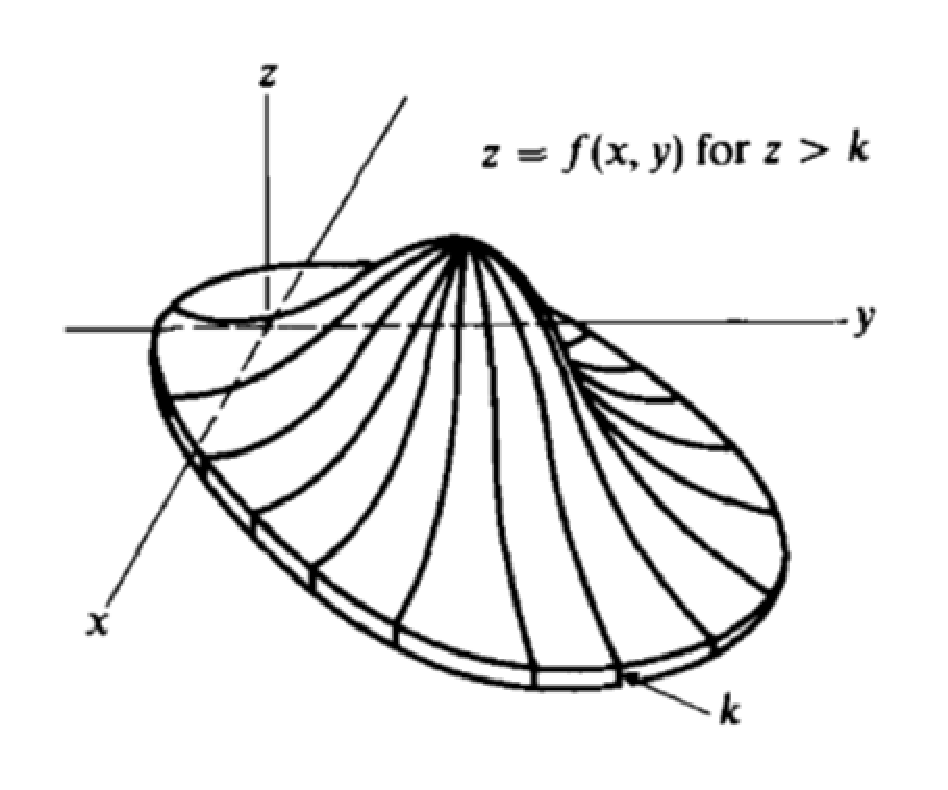
\includegraphics[scale = 0.5]{pictures/bivariate_normal.eps}
\caption{Pravděpodobnostní funkce dvourozměrného normálního rozdělení}
\label{bivariate_normal}
\end{figure}

Příslušná pravděpodobnostní funkce je znározněna na obrázku (\ref{bivariate_normal}). Libovolný řez rovnoběžný s rovinou $xy$ představuje eliptickou křivku, zatímco libovolný řez kolmý na rovninu $xy$ představuje pravděpodobnostní funkci jednorozměrného normálního rozdělení. Pravděpodobnost, že bod $(X,Y)$ leží v regionu $R$ roviny $xy$, je definována jako
\begin{equation*}
P[(X,Y) \in R] = {\int \int}_R f(x,y)dy dx
\end{equation*}

Aby byla pravděpodobnostní funkce dvourozměrného normálního rozdělení pravděpodobnostní funkcí, musí nabývat pouze nezáporných hodnot a musí splňovat podmínku
\begin{equation*}
\int_{-\infty}^{\infty} \int_{-\infty}^{\infty} f(x,y) dy dx = 1
\end{equation*}
Splnění prvního požadavku je patrné ze zběžného pohledu na funkční předpis tohoto pravděpodobnostního rozdělení. Abychom dokázali splnění druhé podmínky, použijeme nejprve substituce
\begin{equation*}
u = \frac{x - E[X]}{\sigma_X}~~~~~v = \frac{y - E[Y]}{\sigma_Y}
\end{equation*}
čímž pravděpodobnostní funkci zjednodušíme do podoby
\begin{equation*}
\int_{-\infty}^{\infty} \int_{-\infty}^{\infty} \frac{1}{2 \pi \sqrt{1 - \rho^2}} e^{-\frac{1}{2(1 - \rho)}(u^2 - 2 \rho u v + v^2)}dv du
\end{equation*}
Doplněním čtverce pro $u$ v exponentu získáváme
\begin{equation*}
\int_{-\infty}^{\infty} \int_{-\infty}^{\infty} \frac{1}{2 \pi \sqrt{1 - \rho^2}}e^{-\frac{1}{2(1 - \rho^2)}[(u - \rho v)^2 + (1 - \rho^2)v^2]}dv du
\end{equation*}
Jestliže dosadíme
\begin{equation*}
w = \frac{u - \rho v}{\sqrt{1 - \rho^2}}~~~~~dw = \frac{du}{\sqrt{1 - \rho^2}}
\end{equation*}
lze výše uvedený integrál rozepsat jako součin dvou jednoduchých integrálů
\begin{equation*}
\int_{-\infty}^{\infty} \frac{1}{\sqrt{2 \pi}}e^{-\frac{w^2}{2}}dw \int_{-\infty}^{\infty} \frac{1}{\sqrt{2 \pi}}e^{-\frac{v^2}{2}}dv
\end{equation*}
které jsou oba rovny jedné.

\subsection{Momentová funkce a momenty}

\begin{theorem}
Sdružená momentová funkce dvourozměrné normální náhodné veličiny $(X,Y)$ je rovna
\begin{equation*}
m(t_1, t_2) = e^{t_1E[X] + t_2E[Y] + \frac{1}{2}(t_1^2 \sigma_X^2 + 2 \rho t_1 t_2 \sigma_X \sigma_Y + t_2^2 \sigma_Y^2)}
\end{equation*}
\end{theorem}

\begin{proof}
Opět dosaďme za $x$ a $y$ veličiny $u$ a $v$, což vede k rovnici
\begin{equation*}
m(t_1, t_2) = e^{t_1E[X] + t_2E[Y]} \int_{-\infty}^{\infty}  \int_{-\infty}^{\infty} e^{t_1 \sigma_X u + t_2 \sigma_Y u} \frac{1}{2 \pi \sqrt{1 - \rho^2}}e^{-\frac{1}{2(1 - \rho^2)}(u^2 - 2 \rho uv + v^2)}dv du
\end{equation*}
Oba exponenty lze sloučit do tvaru
\begin{equation*}
- \frac{1}{2(1 - \rho^2)}\big[u^21 - 2 \rho u v + v^2 - 2(1 - \rho^2)t_1 \sigma_Xu - 2(1 - \rho^2)t_2 \sigma_Y v \big]
\end{equation*}
a doplněním čtverců pro $u$ a $v$ získáme
\begin{gather*}
- \frac{1}{2(1 - \rho^2)}\Big[\big(u - \rho v - (1 - \rho^2)t_1 \sigma_x \big)^2 + (1 - \rho^2)(v - \rho t_1 \sigma_X - t_2 \sigma_Y)^2\\
	-(1 - \rho^2)(t_1^2 \sigma_X^2 + 2 \rho t_1 t_2 \sigma_X \sigma_Y + t_2^2 \sigma_Y^2)\Big]
\end{gather*}
Jestliže použijeme substituce
\begin{equation*}
w = \frac{u - \rho v + (1 - \rho^2)t_1 \sigma_X}{\sqrt{1 - \rho^2}} ~~~~~ z = v - \rho t_1 \sigma_X - t_2 \sigma_Y
\end{equation*}
lze tento výraz dále upravit na
\begin{equation*}
-\frac{1}{2}w^2 - \frac{1}{2}z^2 + \frac{1}{2}(t_1^2 \sigma_X^2 + 2 \rho t_1 t_2 \sigma_X \sigma_Y + t_2^2 \sigma_Y^2)
\end{equation*}
Momentovou funkci pak lze vyjádřit jako
\begin{gather*}
m(t_1, t_2) = e^{t_1 E[X] + t_2 E[X]}e^{\frac{1}{2}(t_1^2 \sigma_X^2 + 2 \rho t_1 t_2 \sigma_X \sigma_Y + t_2^2 \sigma_Y^2)}\int_{-\infty}^{\infty} \int_{-\infty}^{\infty} \frac{1}{2 \pi} e^{-\frac{w^2}{2} - \frac{z^2}{2}}dw dz\\
= e^{t_1 E[X] + t_2 E[Y] + \frac{1}{2}(t_1^2 \sigma_X^2 + 2 \rho t_1 t_2 \sigma_X \sigma_Y + t_2^2 \sigma_Y^2 )}
\end{gather*}
\end{proof}

\begin{theorem}
Jestliže náhodná veličina $(X,Y)$ sleduje dvourozměrné normální rozdělení, pak
\begin{gather*}
\sigma_{X,Y} = \rho \sigma_X \sigma_Y
\end{gather*}
\end{theorem}

\begin{proof}
Sdružený moment $E[X^r Y^s]$ lze získat z  momentové funkce $m(t_1, t_2)$ derivací $r$-krát dle $t_1$ a $s$-krát dle $t_2$ s následným dosazením $t_1 = 0$ a $t_2 = 0$. Kovarianční koeficient $X$ a $Y$ je pak
\begin{gather*}
E[X - E[X]]E[Y - E[Y]] = E[XY - XE[X] - YE[Y] - E[X]E[Y]] = E[XY] - E[X][Y]\\
= \frac{\partial^2}{\partial t_1 \partial t_2}m(t_1, t_2)\Big|_{t_1 = t_2 = 0} - E[X]E[Y] = \rho \sigma_X \sigma_Y
\end{gather*}
\end{proof}

\begin{theorem}
Jestliže má náhodná veličina $(X,Y)$ dvourozměrné normální rozdělení, pak jsou $X$ a $Y$ nezávislé tehdy a jen tehdy, jsou-li $X$ a $Y$ nekorelované.
\end{theorem}

\begin{proof}
Náhodné veličiny jsou nekorelované tehdy a jen tehdy, je-li $\sigma_{X,Y} = 0$ nebo ekvivalentně je-li $\rho_{X,Y} = 0$. Z definice dvourozměrného normálního rozdělení je zřejmé, že je-li $\rho_{X,Y} = 0$, pak se pravděpodobnostní funkce $f_{X,Y}$ stane součinem dvou jednorozměrných normálních rozdělení. Proto $\rho_{X,Y}$ implikuje, že $X$ a $Y$ jsou nezávislé. Víme, že nezávislost náhodných veličin $X$ a $Y$ implikuje jejich nekorelovanost.
\end{proof}

\section{Marginální a podmníněná pravděpodobnostní funkce}

\begin{theorem}
Jestliže $(X,Y)$ sleduje dvourozměrné náhodné rozdělení, pak marginální rozdělení $X$ a $Y$ jsou jednorozměrná normální rozdělení. To znamená, že $X$ je normálně rozdělené se střední hodnotou $E[X]$ a rozptylem $\sigma_X^2$ a $Y$ je normálně rozdělené se střední hodnotou $E[X]$ a rozptylem $\sigma_Y^2$.
\end{theorem}

\begin{proof}
Marginální rozdělení náhodné veličiny $X$ je z definice
\begin{equation*}
f_X(x) = \int_{-\infty}^{\infty} f(x,y)dy
\end{equation*}
S použím substituce $v = \frac{y - E[Y]}{\sigma_Y}$ a doplněním čtverců pro $v$ získáme
\begin{equation*}
f_X(x) = \int_{-\infty}^{\infty} \frac{1}{2 \pi \sigma_X \sqrt{1 - \rho^2}} e^{-\frac{1}{2} \big(\frac{x - E[X]}{\sigma_X} \big)^2 - \frac{1}{2(1 - \rho)^2} \big(v - \rho \frac{x - E[X]}{\sigma_X} \big)^2}dv
\end{equation*}
Následnými substitucemi
\begin{equation*}
w = \frac{v - \rho(x - E[X])/ \sigma_X}{\sqrt{1 - \rho^2}} ~~~~~ dw \frac{1}{\sqrt{1 - \rho^2}}dv
\end{equation*}
lze dokázat
\begin{equation*}
f_X(x) = \frac{1}{\sqrt{2 \pi \sigma_X^2}} e^{-\frac{1}{2}\big(\frac{y - E[Y]}{\sigma_Y} \big)^2}
\end{equation*}
Analogicky lze důkaz provést také pro $f_Y(y)$.
\end{proof}
\begin{theorem}
Jestliže $(X,Y)$ sleduje dvourozměrné normální rozdělení, pak podmíněná pravděpodobnostní funkce náhodné veličiny $X$ pro $Y = y$ sleduje normální rozdělení se střední hodnotou $E[X] + \rho \frac{\sigma_X}{\sigma_Y}(y - E[Y])$ a rozptylem $\sigma_X^2(1 - \rho^2)$. Podobně podmíněná pravděpodobnostní funkce náhodné veličiny $Y$ pro $X = x$ sleduje normální rozdělení se střední hodnotou $E[Y] + \rho \frac{\sigma_Y}{\sigma_X}(x - E[X])$ a rozptylem $\sigma_Y^2(1 - \rho^2)$.
\end{theorem}

\begin{proof}
Podmíněné pravděpodobnostní funkce lze odvodit s pomocí sdružené a marginální pravděpodobnostní funkce.
\begin{equation*}
f_{X|Y}(x|y) = \frac{f(x,y)}{f_Y(y)}
\end{equation*}
Dosazením a následnými úpravami získáme
\begin{equation*}
f_{X|Y}(x|y) = \frac{1}{\sqrt{2 \pi} \sigma_X \sqrt{1 - \rho^2}}e^{-\frac{1}{2 \sigma_X^2(1 - \rho^2)}\big[x - E[X] - \frac{\rho \sigma_X}{\sigma_Y}(y - E[Y]) \big]^2}
\end{equation*}
což je jednorozměrné normální rozdělení se střední hodnotou $E[X] + \rho \frac{\sigma_X}{\sigma_Y}(y - E[Y])$ a rozptylem $\sigma_X^2(1 - \rho^2)$. Analogicky lze odvodit také $f_{Y|X}(y|x)$.
\end{proof}

Již dříve jsme zmínili, že v případě podmíněného rozdělení nazýváme střední hodnotau náhodné veličiny regresní křivkou. Ve výše uvedeném případě je regrese $X$ pro $Y = y$ rovna $E[X] + \rho \frac{\sigma_X}{\sigma_Y}(y - E[Y])$, což je lineární funkce veličiny $y$.

\begin{figure}[htp]
\centering
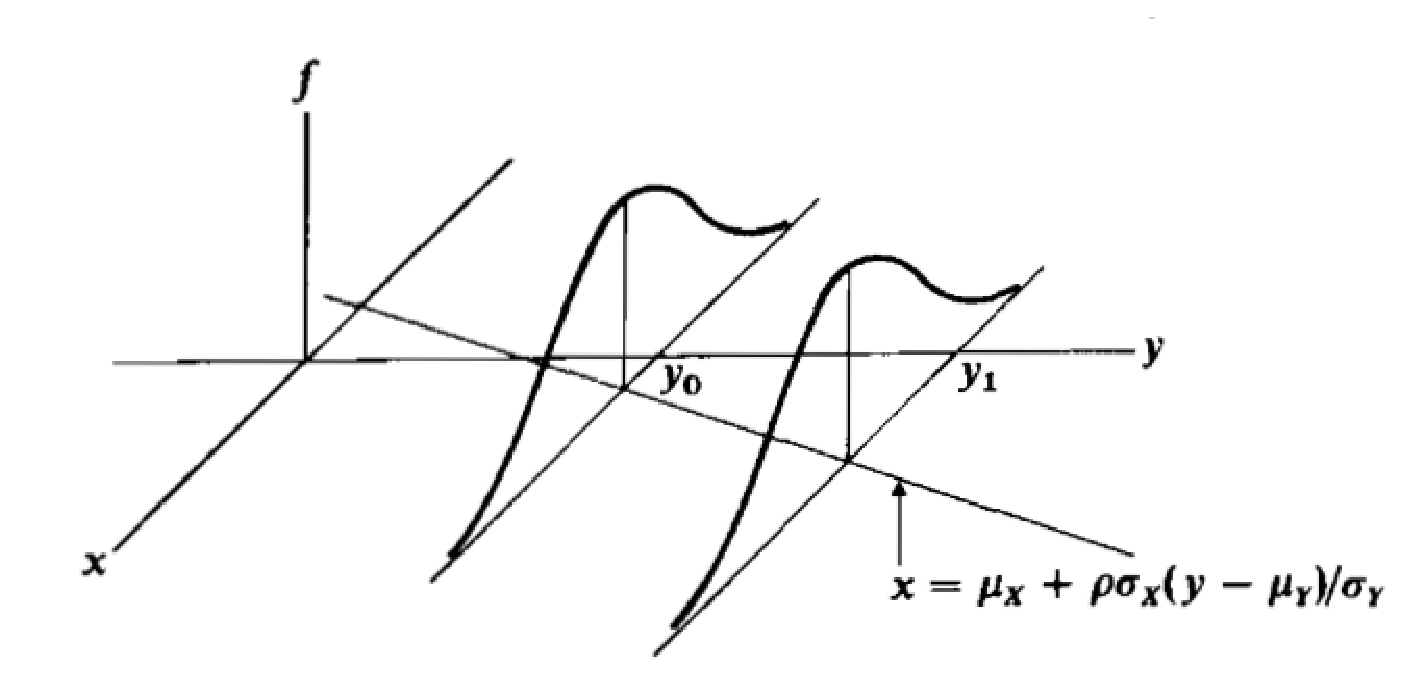
\includegraphics[scale = 0.5]{pictures/bivariate_normal_regression.eps}
\caption{Regresní křivka pro podmíněné dvourozměrné normální rozdělení}
\label{bivariate_normal_regression}
\end{figure}  
 

